\chapter{Opis implementacije}
Implementacija uglavnom slijedi algoritam HERA \engl{Highly Efficient Repeat Assembly} opisan u radu \citep{Du345983} uz nekoliko manjih modifikacija. Algoritam se sastoji od tri glavnih koraka. Prvo se gradi graf preklapanja u kojem se traže putevi između contig-a. Nakon što su pronađeni mogući putevi, za svaki par contig-a se traži reprezentativna sekvenca te se u konačnici sastavlja jedna sekvenca između povezanih contig-a.

Alat Minimap2, ukoliko pronađe preklapanje između dvije sekvence (očitanje ili contig), da informacije o indeksima početka i kraja preklapanja za obje sekvence. Prvi korak je odbacivanje preklapanja koja zadovoljavaju barem jedan od sljedećih uvjeta:

\begin{itemize}
\item preklapanje je između dvije iste sekvence,
\item preklapanje u kojem jedna sekvenca u potpunosti sadrži drugu,
\item SI \engl{sequence identity} mjera je ispod određene granice (primjerice 40\%).
\end{itemize}

\begin{figure}[htb]
\centering
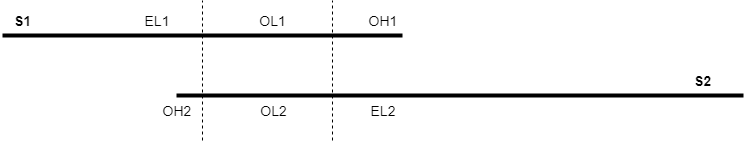
\includegraphics[width=\textwidth]{img/overlap.png}
\caption{Primjer preklapanja između S1 i S2}
\label{fig:overlap}
\end{figure}

Za preostale sekvence se računaju mjere preklapanja i produživanja. Na slici \ref{fig:overlap} je prikazano preklapanje između sekvenca $S_1$ i $S_2$ gdje se sekvenca $S_2$ nalazi nakon sekvence $S_1$. U sredini između isprekidanih linija je regija preklapanja čija je duljina $OL_1$ i $OL_2$, ovisno koju sekvencu gledamo, a izvana su $OH$ \engl{overhang length} i $EL$ \engl{extension length}. Koristeći navedene duljine, računa se mjera preklapanja $OS$ i mjere produživanja $ES_1$ i $ES_2$ prema izrazima \ref{eq:os} - \ref{eq:es2}. Pri tome je potrebno voditi računa preklapaju li se sekvence na istim lancima ili na suprotnim. Primjerice da se $S_1$ i $S_2$ preklapaju na suprotnim lancima, potrebno bi bilo zamijeniti vrijednosti $OH_2$ i $EL_2$.

\begin{equation}
OS = \frac{(OL_1 + OL_2) * SI}{2}
\label{eq:os}
\end{equation}
\begin{equation}
ES_1 = OS + \frac{EL_1}{2} - \frac{OH_1 + OH_2}{2}
\label{eq:es1}
\end{equation}
\begin{equation}
ES_2 = OS + \frac{EL_2}{2} - \frac{OH_1 + OH_2}{2}
\label{eq:es2}
\end{equation}

\section{Graf preklapanja}
Nakon što su sve mjere izračunate može se izgraditi graf preklapanja. Čvorovi u grafu predstavljaju contig-e i očitanja, a grane preklapanja, s time da grana može biti povezana na glavu ili rep čvora. Drugim riječima, svaki čvor ima svoje prefikse i sufikse. Sljedeći korak je traženje puteva između dva contig-a koji se obavlja pretraživanjem u dubinu \engl{DFS} uz nekoliko pravila. Postupak kreće iz svakog contig-a i zaustavlja se kada dođe do očitanja koje je povezano s drugim contig-om ili je trenutni put veći od maksimalne dopuštene duljine. Dodatno ograničenje je da se jedno očitanje ne može više puta pojaviti u istom putu.

Za izgradnju puteva koriste se tri pristupa. Prvi pristup iz početnog contiga izabere sve sufikse, ali za svako sljedeće produživanje bira ono koje ima najveću mjeru preklapanja $OS$. Ukoliko se dođe do čvora koji nema produživanja, vraća se jedan korak nazad i bira sljedeće najbolje produživanje. Drugi pristup radi isto kao prvi jedino koristi mjeru produživanja $ES$. Konačno, treći pristup nasumično bira produživanja proporcionalno mjeri produživanja $ES$, s time da je potrebno odrediti koliko puta će se iz svakog contig-a pokušati pronaći put ovom metodom. Po završteku postupka pronalaženja puteva između contig-a potrebno je samo odbaciti duplikate i moguće je prijeći na sljedeći korak algoritma.

\section{Stevo}

\section{Mihaela}